\section{Palíndromos}

\subsection{MT Determinista de 1 cinta}

\subsubsection*{Diseño propuesto}
El algoritmo de resolución es el siguiente:

\begin{itemize}
    \item Ciclo:
    \begin{enumerate}[1.]
        \item Si no hay ninguna letra, poner un \texttt{1} y \textbf{parar}.
        \item Borrar una letra en el extremo izquierdo.
        \item Buscar la letra correspondiente en el extremo derecho.
        \item Si la letra coincide:
        \begin{enumerate}[1.]
            \item Borrarla.
            \item Volver al extremo izquierdo.
        \end{enumerate}
        \item En caso contrario:
        \begin{enumerate}[1.]
            \item Volver al extremo izquierdo, borrando todas las letras.
            \item Poner un \texttt{0} y \textbf{parar}.
        \end{enumerate}
    \end{enumerate}
\end{itemize}

La implementación en JFLAP sería la siguiente:

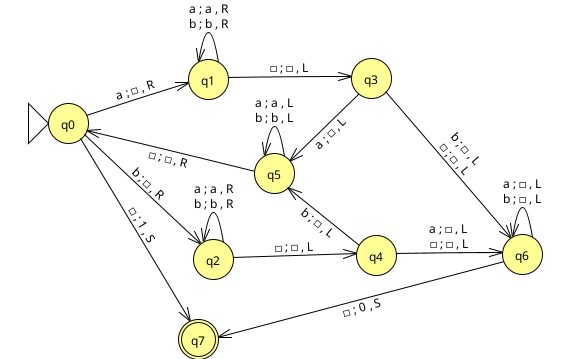
\includegraphics[width=\textwidth]{MT-0A.png}


\subsubsection*{Peor caso}
El peor caso sería cuando es un palíndromo, dado que en el momento en el que una letra no coincida, deja de buscar el resto de letras. Dentro de los palíndromos, el peor caso es cuando es un palíndromo de tamaño par, ya que tiene que hacer una comprobación extra.

\subsubsection*{Análisis empírico}

Realizamos el análisis empírico en el peor caso, tomando como $N$ el tamaño de la palabra, y midiendo el número de pasos realizados para resolver el problema:

\begin{table}[h]
    \centering
    \begin{tabular}{lcc}
        Entrada & $N$ & Pasos \\
        \hline
        $\lambda$      & 0  & 1  \\
        aa             & 2  & 6  \\
        abba           & 4  & 15 \\
        abaaba         & 6  & 28 \\
        aaabbaaa       & 8  & 45 \\
        bbaabbaabb     & 10 & 66 \\
        bbbbbaabbbbb   & 12 & 91
    \end{tabular}
\end{table}


\subsubsection*{Evaluación analítica}
Para obtener el coste computacional del algoritmo, aplicaremos Diferencias Finitas:

\begin{table}[h]
    \centering
    \begin{tabular}{|l|c|c|c|c|c|c|c|}
        \hline
        $N$ & \textbf{0} & \textbf{2} & \textbf{4} & \textbf{5} & \textbf{8} & \textbf{10} & \textbf{12} \\ \hline
        Pasos & \textbf{1} & \textbf{6} & \textbf{15} & \textbf{28} & \textbf{45} & \textbf{66} & \textbf{91} \\ \hline
        \hline
        $A(N) = T(N) - T(N-2)$ &    &  5 &  9 & 13 & 17 & 21 & 25 \\ \hline
        $B(N) = A(N) - A(N-2)$ &    &  4 &  4 &  4 &  4 &  4 &    \\ \hline
        $C(N) = B(N) - B(N-2)$ &    &    &  0 &  0 &  0 &  0 &    \\ \hline
    \end{tabular}
\end{table}

Al ser constantes las diferencias finitas segundas, y nulas las terceras, podemos aproximar $T(N)$ con un polinomio de segundo orden, es decir, $T(N) = aN^2 + bN + c$.\\

Para obtener los valores de $a$, $b$, y $c$, usaremos valores de $N$ y $T(N)$ obtenidos en la evaluación empírica:

\begin{subequations}
    \begin{gather}
        N = 0,\ T(0) = 1 \rightarrow c = 1 \\
        N = 2,\ T(0) = 6 \rightarrow 4a + 2b + c = 6 \\
        N = 4,\ T(0) = 15 \rightarrow 16a + 4b + c = 6
    \end{gather}
\end{subequations}

Resolviendo, $a=\frac{1}{2}$ y $b=\frac{3}{2}$, por lo que:

\begin{equation}
    T(N) = 2N^2 + 6N + 2
\end{equation}


